\documentclass[UTF8]{ctexart}
\usepackage{graphicx}
\title{AVL树和跳表插入性能测试}

\author{\\
\\
\\
\\
\\
\\
\\
\\
\\
\\
\\
杨景凯\\
520021910550
  }
\date{\today}
\begin{document}
\maketitle
\clearpage
\tableofcontents
\clearpage
\section{AVL树随机插入测试}
\subsection{实验说明}
此部分针对于AVL树进行了不同个数的元素的插入测试。

随机生成一组插入序列,插入元素的个数分别为 50,100,500,1000,2000。

得到了插入元素个数和插入时间的关系。
\subsection{实验表格}
\begin{center}
    \begin{tabular}{|c|c|c|c|c|c|}
        \hline
        个数&	50&	100&	500&	1000&	2000\\
        \hline
        时间&	0.000013&	0.000023&	0.000112&	0.000232&	0.000493\\
        \hline
    \end{tabular}
\end{center}
\subsection{实验图表}
\begin{center}
    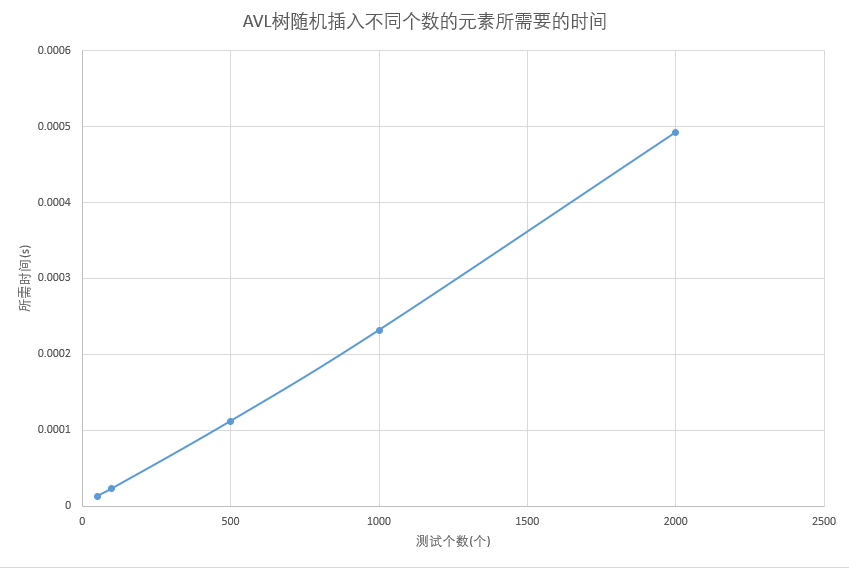
\includegraphics[scale=0.5]{AVLinsert.png}
\end{center}
\section{AVL树条件插入测试}
\subsection{实验说明}
此部分针对AVL树与跳表,进行了不同条件的插入测试。

针对插入元素的个数为 2000 的 AVL 树和跳表,对比下列三种情况它们的插入所需时间的差异。

1)顺序插入(后一个插入的 key 恒大于前一个值)

2)随机插入(随机生成插入序列)

3)逆序插入(后一个插入的 key 恒小于前一个值)

得到了两者在不同条件下的插入时间。
\subsection{实验表格}
\begin{center}
    \begin{tabular}{|c|c|c|c|}
        \hline
        状况&	顺序&	随机&	逆序\\
        \hline
        AVL树&	0.000437&	0.000493&	0.000411\\
        \hline
        跳表&	0.001554&	0.001608&	0.001361\\
        \hline
    \end{tabular}
\end{center}
\subsection{实验图表}
\begin{center}
    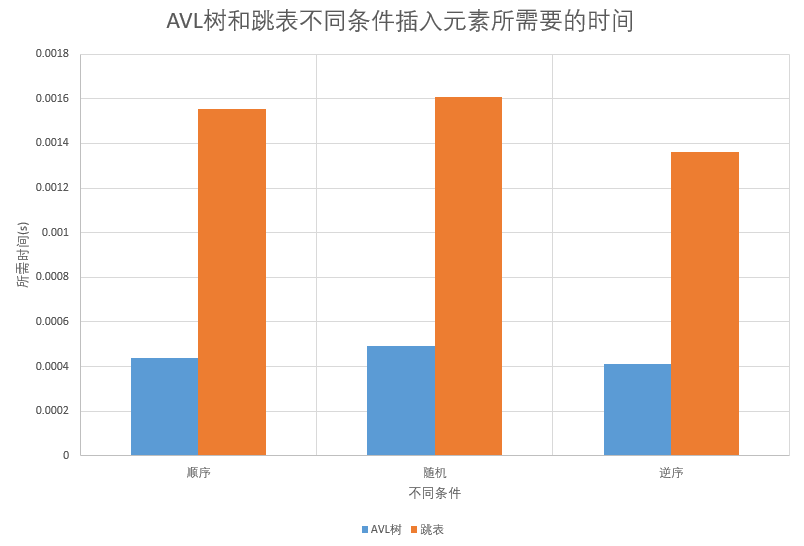
\includegraphics[scale=0.5]{Conditioninsert.png}
\end{center}
\section{结果分析}
\subsection{理论分析}
\subsubsection{实验一}
对于AVL树来说,插入时间$T \sim n\log n $,因此,随着插入元素增加,插入时间接近于线性增加,略微有上扬的趋势。

通过实验一的表格和图表可以证明这一点,因此实验结果与理论吻合。
\subsubsection{实验二}
AVL树对数据排序类型不敏感,因此在顺序,逆序和随机上所用时间差距不大(随机数据有生成随机数的影响)。

跳表对数据排序类型较敏感,逆序比顺序所需时间短,但是差异不大。

通过实验二的表格和图表可以证明这一点,因此实验结果与理论吻合。

但是,理论上跳表和AVL树插入时间应该接近,但是实验出现了较为明显的差距。

通过分析,我认为是跳表有计算生成随机数和每个跳表数据块大量数据拷贝的缘故。这导致了跳表要慢于AVL树。
\subsection{选择}
在顺序插入大量数据时,我选择AVL树。因为此时跳表每次都在末尾插入数据,时间复杂度下界是$O(n\log n)$,而AVL树顺序插入时间复杂度为$O(n\log n)$。

在随机插入大量数据时,我认为两个都可以选择,此时两个的平均时间复杂度均为$O(n\log n)$。

在逆序插入大量数据时,我选择跳表。因为跳表每次都可以在开头插入数据,使得平均时间复杂度由$O(n\log n)$降为$O(n)$,而AVL树顺序插入时间复杂度为$O(n\log n)$。
\end{document}